% Fig. 1 source: system and threat model. Compile with pdflatex -> fig_system.pdf
% (Overleaf users: images/fig_system.pdf is already compiled; this file is only for edits.)
\documentclass[tikz,border=2pt]{standalone}
\usepackage{mathptmx}
\usetikzlibrary{arrows.meta,positioning,calc}
\definecolor{atk}{HTML}{C0392B}
\definecolor{ink}{HTML}{222222}
\definecolor{fillA}{HTML}{EAF1F8}
\definecolor{fillB}{HTML}{F4F4F1}
\begin{document}
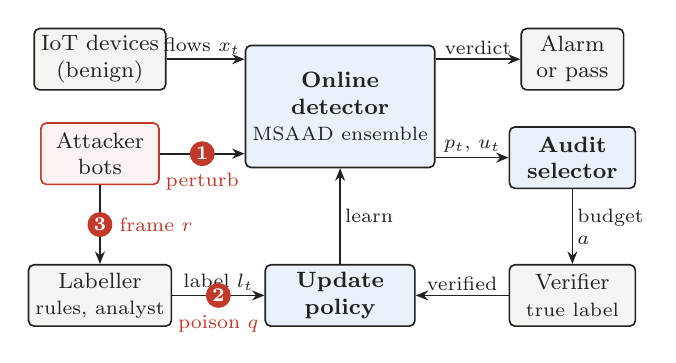
\begin{tikzpicture}[
  font=\footnotesize, >={Stealth[length=4.5pt,width=3.6pt]}, line width=0.6pt, draw=ink, text=ink,
  box/.style={draw, rounded corners=2pt, align=center, inner sep=2.5pt, minimum height=0.78cm},
  core/.style={box, fill=fillA},
  side/.style={box, fill=fillB},
  bad/.style={box, draw=atk, fill=atk!6},
  flow/.style={->},
  lab/.style={font=\scriptsize, inner sep=1.5pt},
  num/.style={circle, fill=atk, text=white, font=\scriptsize\bfseries, inner sep=0.6pt, minimum size=9pt},
  atklab/.style={font=\scriptsize, text=atk, inner sep=1pt}
]
% ---- traffic sources
\node[side, minimum width=1.5cm] (dev) at (0,3.0) {IoT devices\\(benign)};
\node[bad,  minimum width=1.5cm] (bot) at (0,1.8) {Attacker\\bots};
% ---- detector and verdict
\node[core, minimum width=2.2cm, minimum height=1.55cm] (det) at (3.05,2.4) {\textbf{Online}\\\textbf{detector}\\{\scriptsize MSAAD ensemble}};
\node[side, minimum width=1.3cm] (out) at (6.0,3.0) {Alarm\\or pass};
% ---- label channel
\node[side, minimum width=1.6cm] (lab) at (0,0) {Labeller\\{\scriptsize rules, analyst}};
\node[core, minimum width=1.9cm] (pol) at (3.05,0) {\textbf{Update}\\\textbf{policy}};
\node[core, minimum width=1.6cm] (sel) at (6.0,1.75) {\textbf{Audit}\\\textbf{selector}};
\node[side, minimum width=1.6cm] (ver) at (6.0,0) {Verifier\\{\scriptsize true label}};
% ---- data path
\draw[flow] (dev.east) -- node[lab, above, pos=0.45] {flows $x_t$} (det.west |- dev.east);
\draw[flow] (bot.east) -- (det.west |- bot.east);
\draw[flow] (det.east |- out.west) -- node[lab, above] {verdict} (out.west);
\draw[flow] (det.east |- sel.west) -- node[lab, above] {$p_t$, $u_t$} (sel.west);
\draw[flow] (bot.south) -- (lab.north -| bot.south);
\draw[flow] (lab.east) -- node[lab, above] {label $l_t$} (pol.west);
\draw[flow] (sel.south) -- node[lab, right, align=left] {budget\\$a$} (ver.north);
\draw[flow] (ver.west) -- node[lab, above] {verified} (pol.east);
\draw[flow] (pol.north) -- node[lab, right] {learn} (det.south);
% ---- attacker entry points (explained in the caption)
\node[num] (n1) at ($(bot.east)!0.5!(det.west |- bot.east)$) {1};
\node[atklab, below=1pt of n1] {perturb};
\node[num] (n2) at ($(lab.east)!0.5!(pol.west)$) {2};
\node[atklab, below=1pt of n2] {poison $q$};
\node[num] (n3) at ($(bot.south)!0.5!(lab.north)+(0,0)$) {3};
\node[atklab, right=1pt of n3] {frame $r$};
\end{tikzpicture}
\end{document}
